%!TEX root = ../report.tex
\documentclass[report.tex]{subfiles}
\begin{document}
    \chapter{Methodology}

    How you are planning to test/compare/evaluate your research.
    Criteria used.

        % Dont know where to put DATASET related content
    % One entire section could be my comparative study on multimodal dataset
    \section{Available Datasets}

    \begin{itemize}
        \item The majority of deep multimodal perception approaches rely on supervised learning, and therefore necessitate multimodal datasets with labeled ground truth for training deep neural networks. While several multimodal datasets are available, many of these datasets are collected under clear weather conditions or do not include all sensors, such as cameras, LiDAR, and radar. Unfortunately, the availability of multimodal datasets collected under adverse weather conditions with all three sensors is limited. Table 1 summarizes some of the available multimodal datasets for evaluating the performance of deep multimodal perception techniques in adverse weather conditions. Of these datasets, only the recently released K-Radar \cite{Paek2022Jun} incorporates a high-resolution 4D-radar sensor. In the table, C-R-L-N-F denotes the Camera, Radar, LiDAR, Near-infrared, and Far-infrared sensors, respectively.
            \begin{table}[h]
                \centering
                \caption{List multimodal datasets with adverse weather conditions}
                \label{tab:my-table}
                \begin{tabular}{|l|l|l|l|}
                    \hline
                    \textbf{Name}       & \textbf{Sensors} & \textbf{Reference}               & \textbf{Year} \\ \hline
                    DENSE               & CRLNF            & \cite{bijelic2020seeing}    & 2020          \\ \hline
                    EU Long-term        & CRL              & \cite{yan2020eu}            & 2020          \\ \hline
                    nuScenes            & CRL              & \cite{caesar2020nuscenes}   & 2020          \\ \hline
                    The Oxford RobotCar & CRL              & \cite{barnes2020oxford}     & 2020          \\ \hline
                    RADIATE             & CRL              & \cite{sheeny2021radiate}    & 2021          \\ \hline
                    K-Radar             & CRL              & \cite{Paek2022Jun}          & 2022          \\ \hline
                    aiMotive            & CRL              & \cite{matuszka2022aimotive} & 2022          \\ \hline
                    Boreas              & CRL              & \cite{burnett2022boreas}    & 2022          \\ \hline
                    WADS                & CRLNF            & \cite{kurup2022winter}      & 2023          \\ \hline
                \end{tabular}
            \end{table}

            \begin{figure}[h]
                \centering
                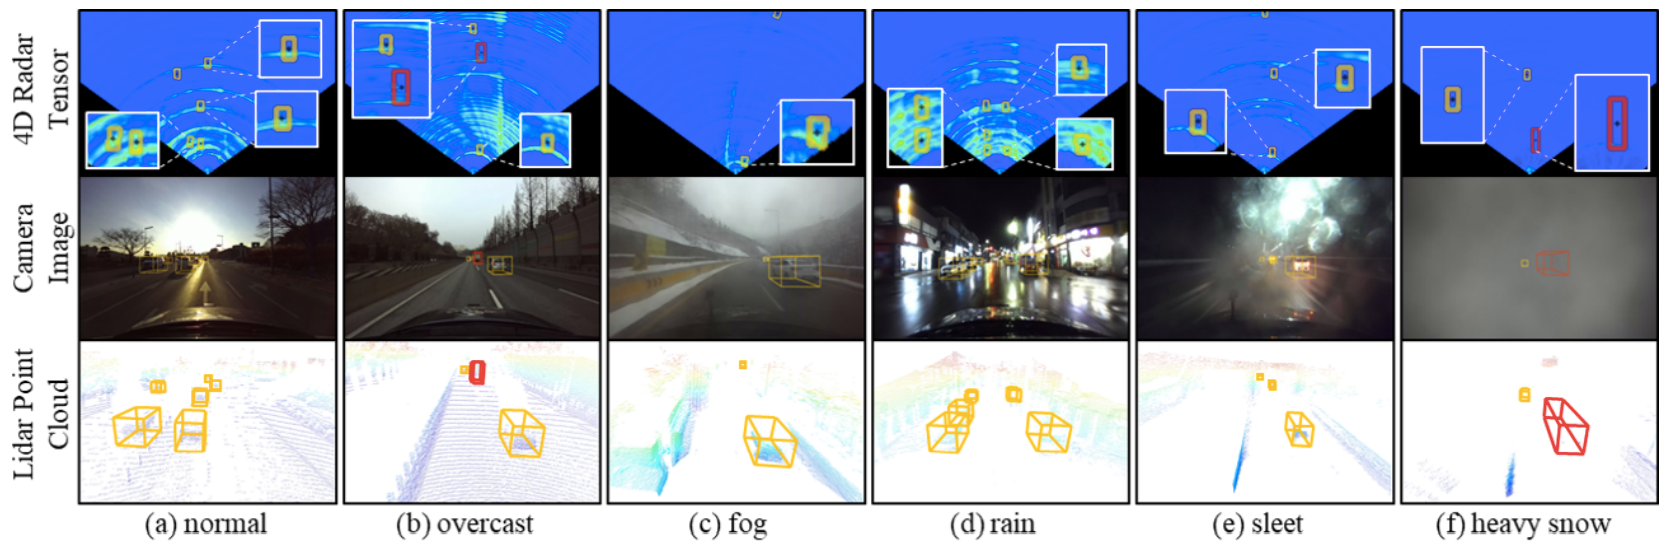
\includegraphics[width=1.0\textwidth]{images/all_sensors_in_adverse_weather.png}
                \caption{\centering Samples of K-Radar datasets for various weather conditions \cite{Paek2022Jun}}
                \label{fig:all_sensors_in_adverse_weather}
            \end{figure}
        \end{itemize}

    \section{Setup}

    \section{Experimental Design}

    \section{Evaluation Metrics}

    

\end{document}
